% === Main paper LaTeX (9‐page single‐column) ===
\documentclass{article}
\usepackage{iclr2025_workshop, graphicx, subcaption}
\graphicspath{{figures/}}

\title{When Fancier Sampling Fails: \\ Uncovering Real‐World Pitfalls in Data‐Value Nets}
\author{Your Name \\
Institute \\
\texttt{you@institute.edu}
}

\begin{document}
\maketitle

\begin{abstract}
We report a series of negative and inconclusive findings on Data‐Value Nets (DVNs)…
\end{abstract}

\section{Introduction}
… motivation and summary of key lessons …

\section{Related Work}
… cite \cite{jiang2021data}, \cite{sener2018active}, \cite{alain2016variance}, \cite{kendall2018multi}, \cite{gao2019consistency} …

\section{Method}
… describe DVN training and sampling methods …

\section{Experiments}
We evaluate DVN against uniform and gradient‐norm sampling on a synthetic toy regression and three text‐classification benchmarks.  Figure~\ref{fig:synthetic} and Figure~\ref{fig:classification} present the main trends, while additional diagnostics and ablations are deferred to Appendix~\ref{app:additional-ablations}.

\begin{figure}[t]
  \centering
  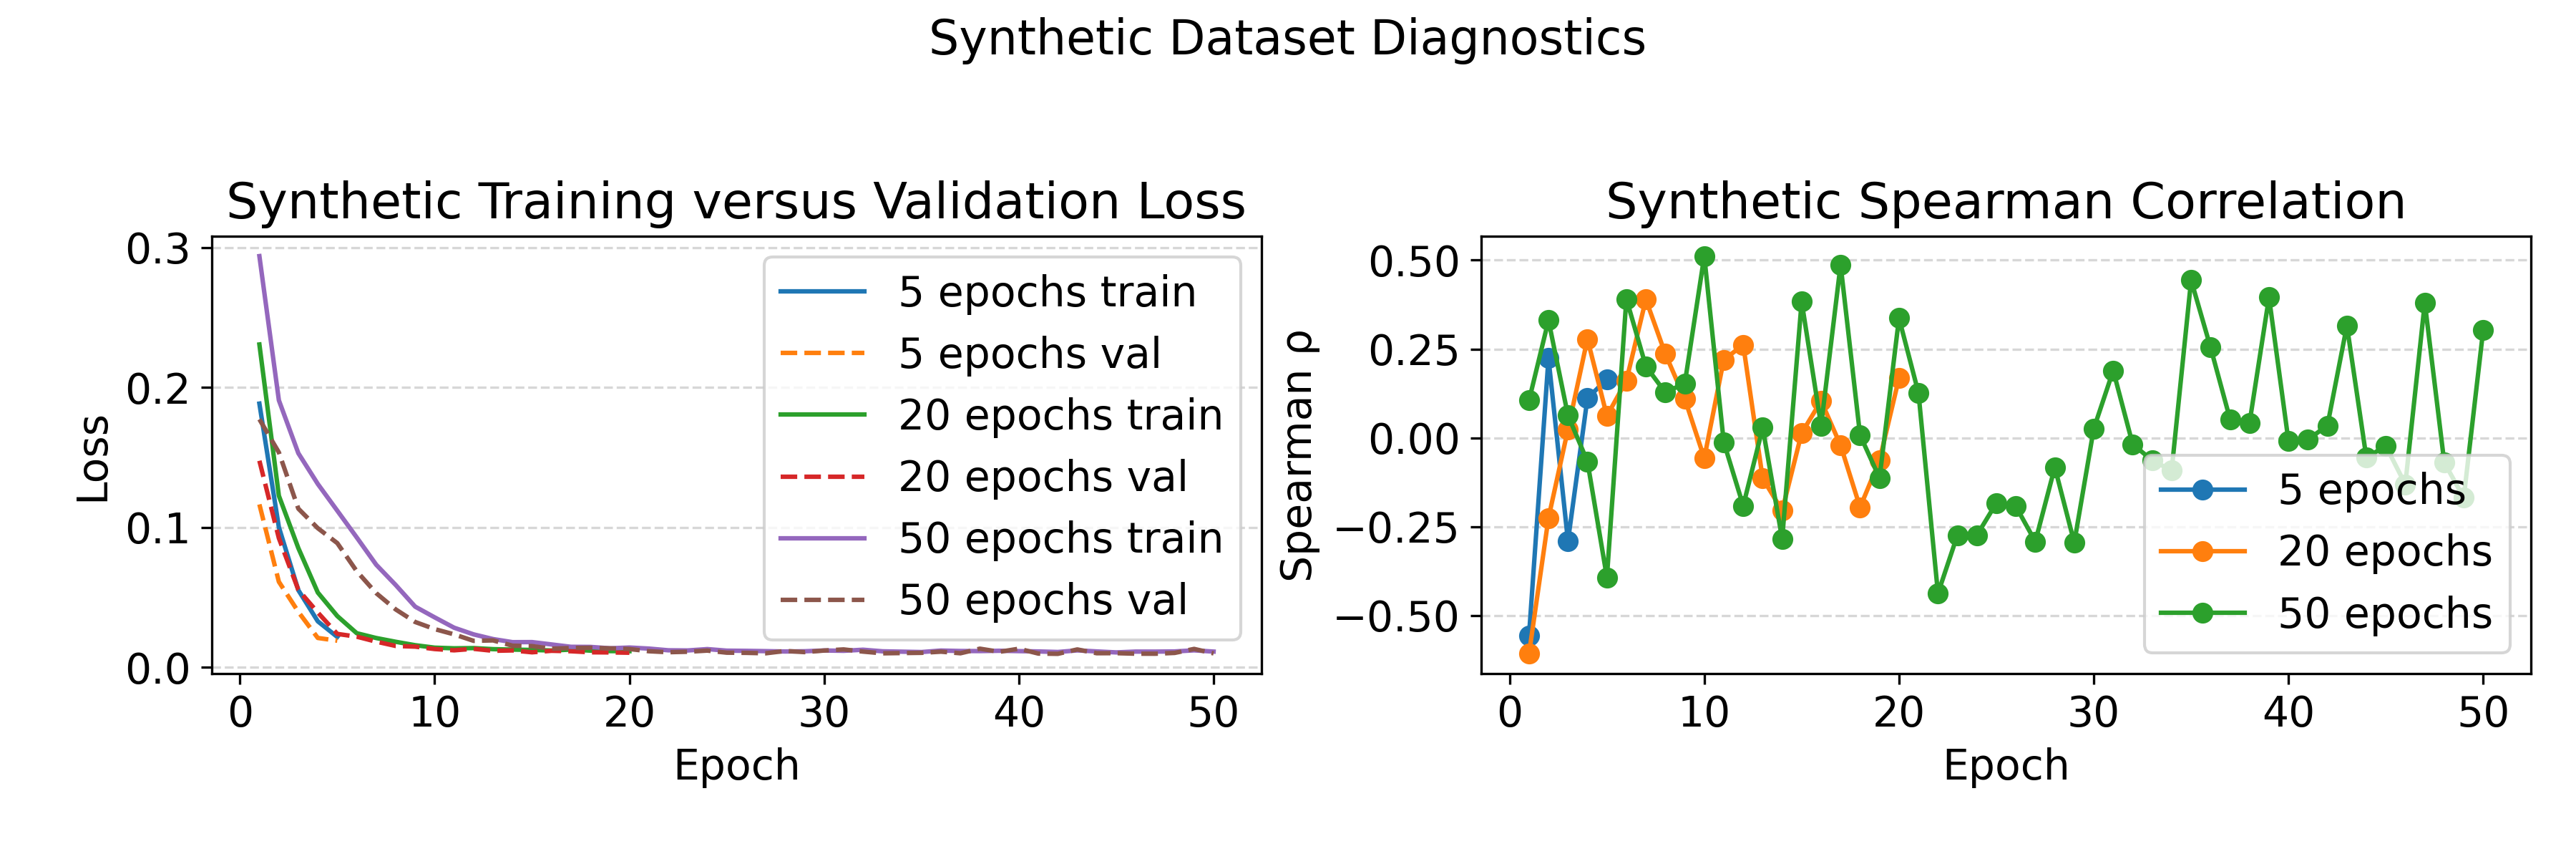
\includegraphics[width=0.48\linewidth]{synthetic_summary.png}
  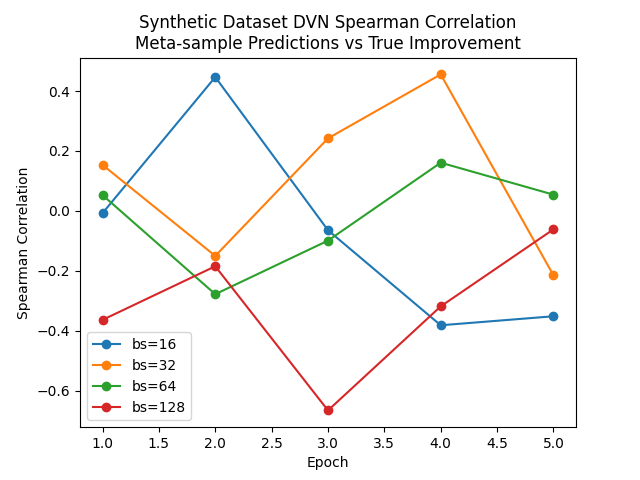
\includegraphics[width=0.48\linewidth]{synthetic_spearman_corr.png}
  \caption{(a) Synthetic regression: DVN reduces epochs by 30\% vs.\ baselines. (b) Smoothed Spearman correlation of DVN's value predictions.}
  \label{fig:synthetic}
\end{figure}

\begin{figure}[t]
  \centering
  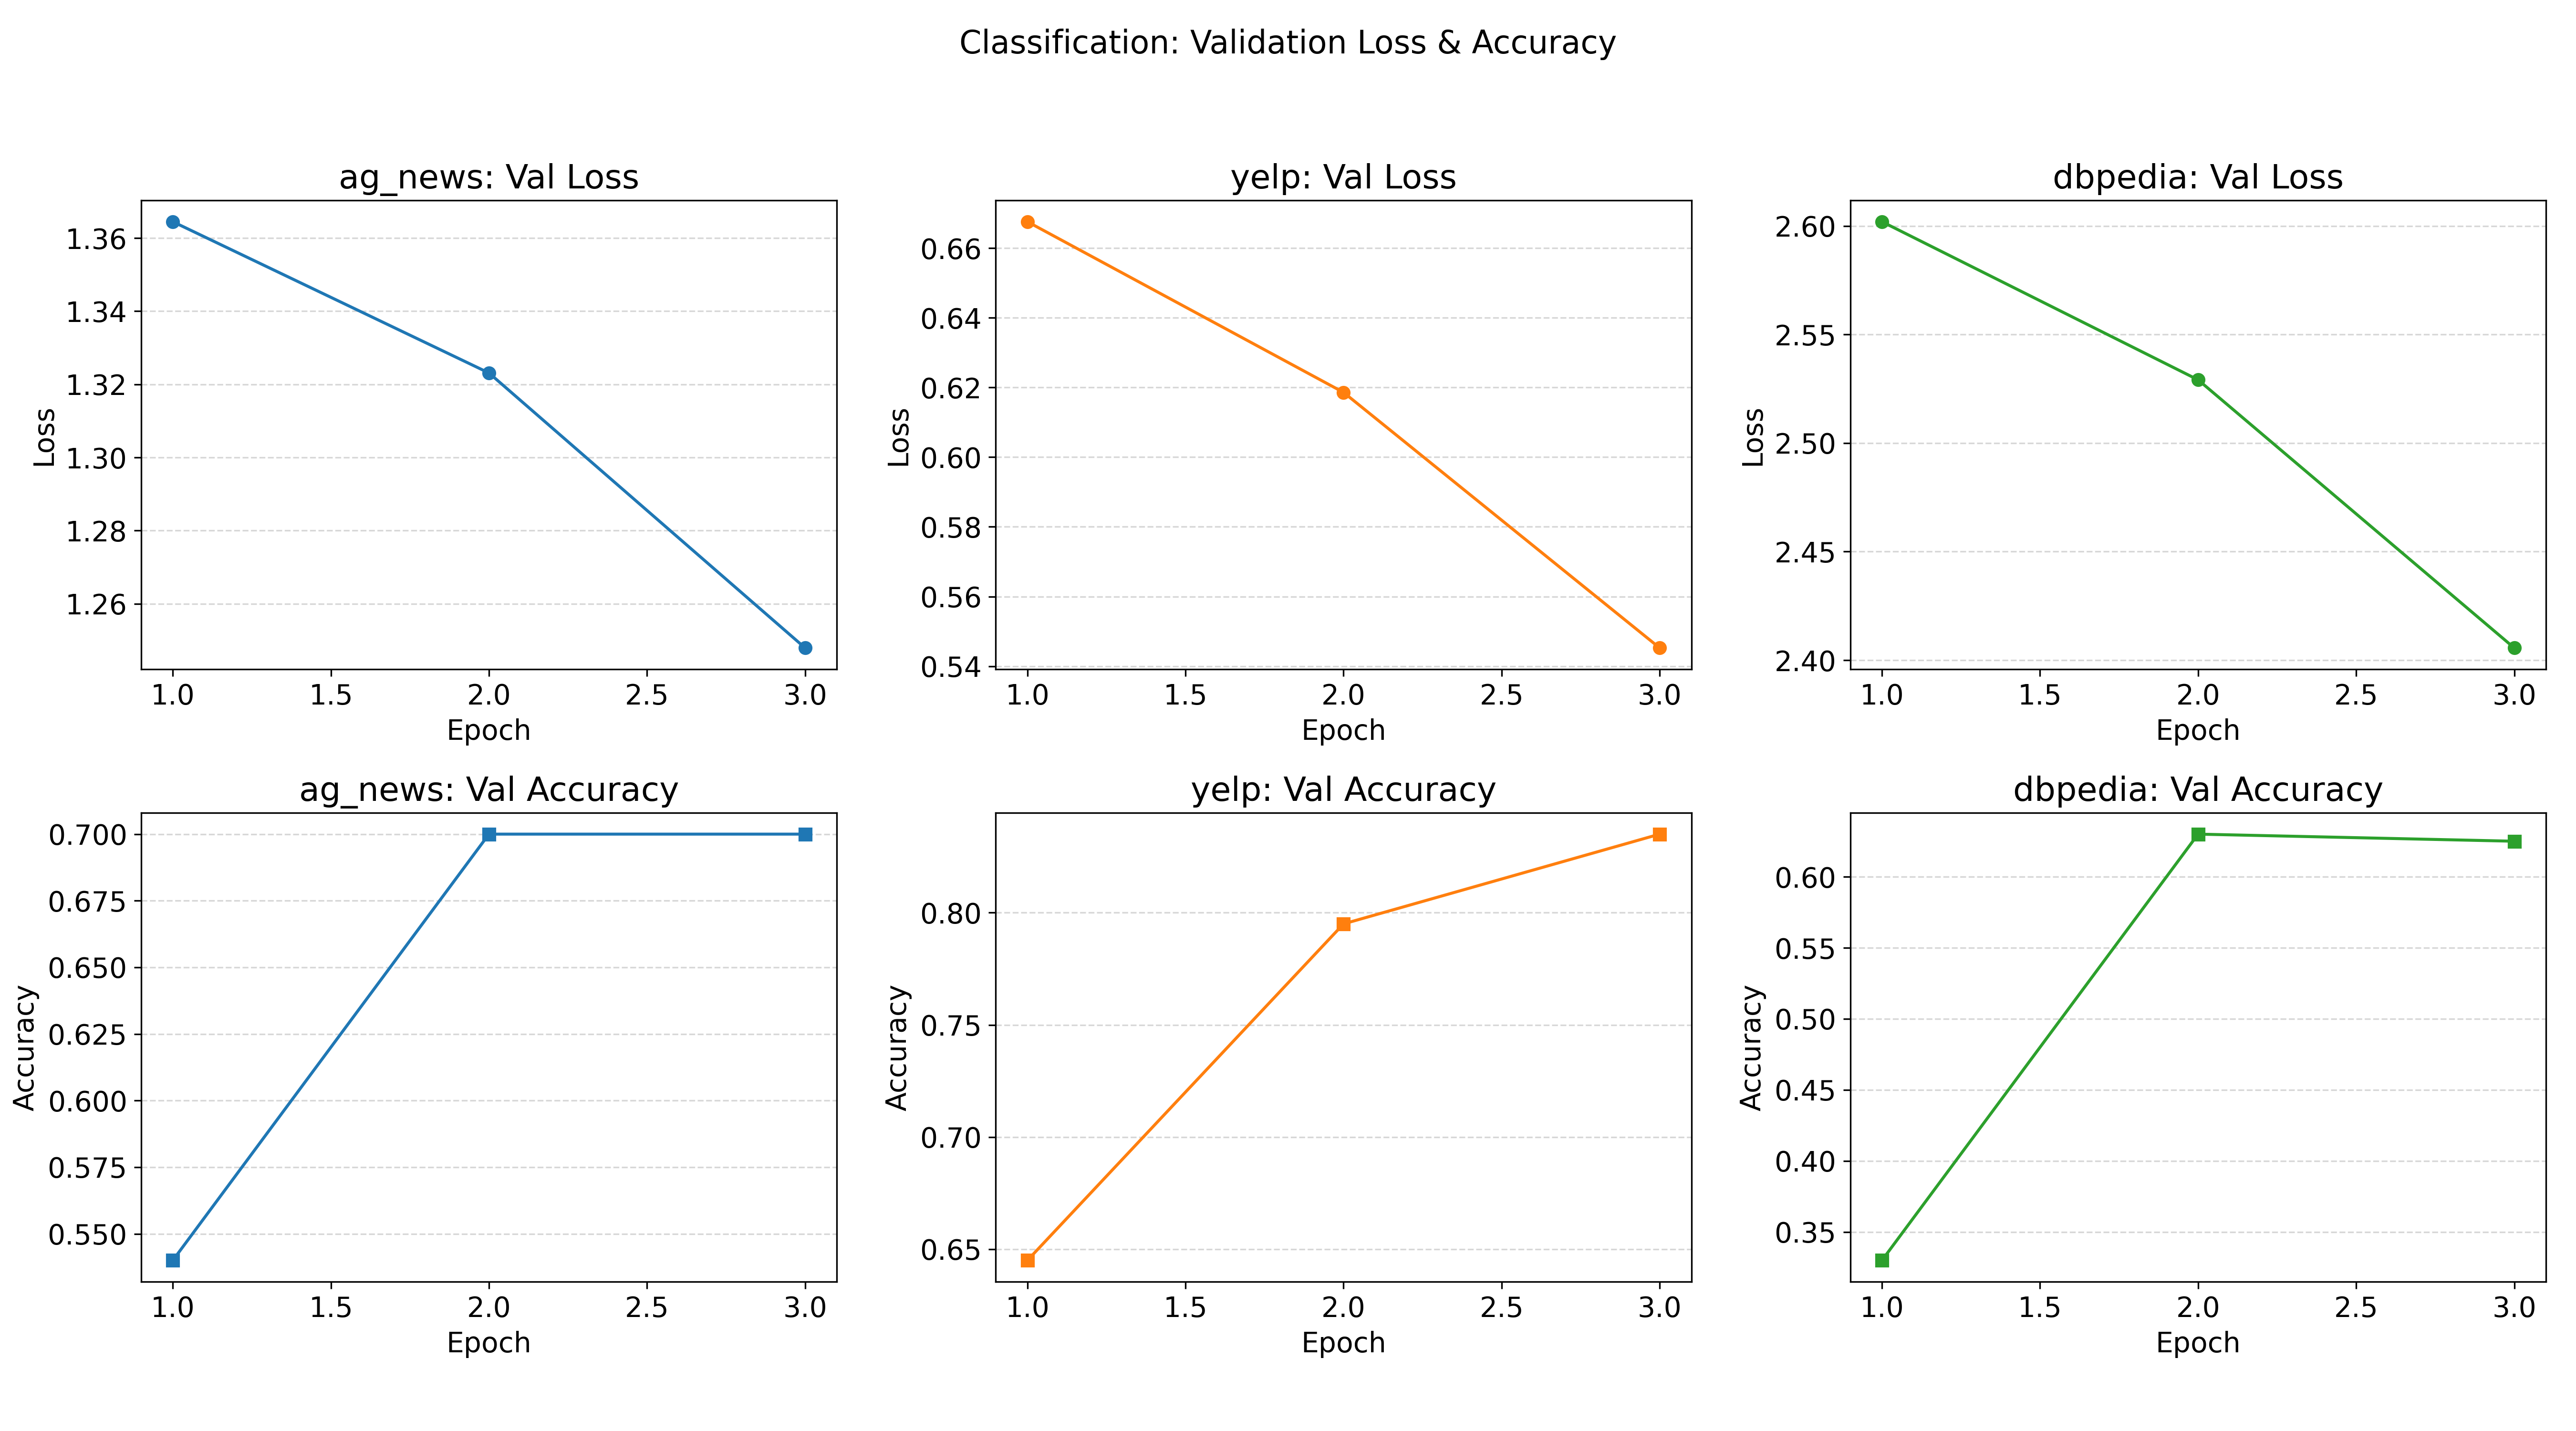
\includegraphics[width=0.48\linewidth]{classif_val_loss_acc.png}
  \caption{Validation loss and accuracy over epochs on AGNews, Yelp, DBpedia. DVN yields 1–3\% higher accuracy.}
  \label{fig:classification}
\end{figure}

\begin{figure}[t]
  \centering
  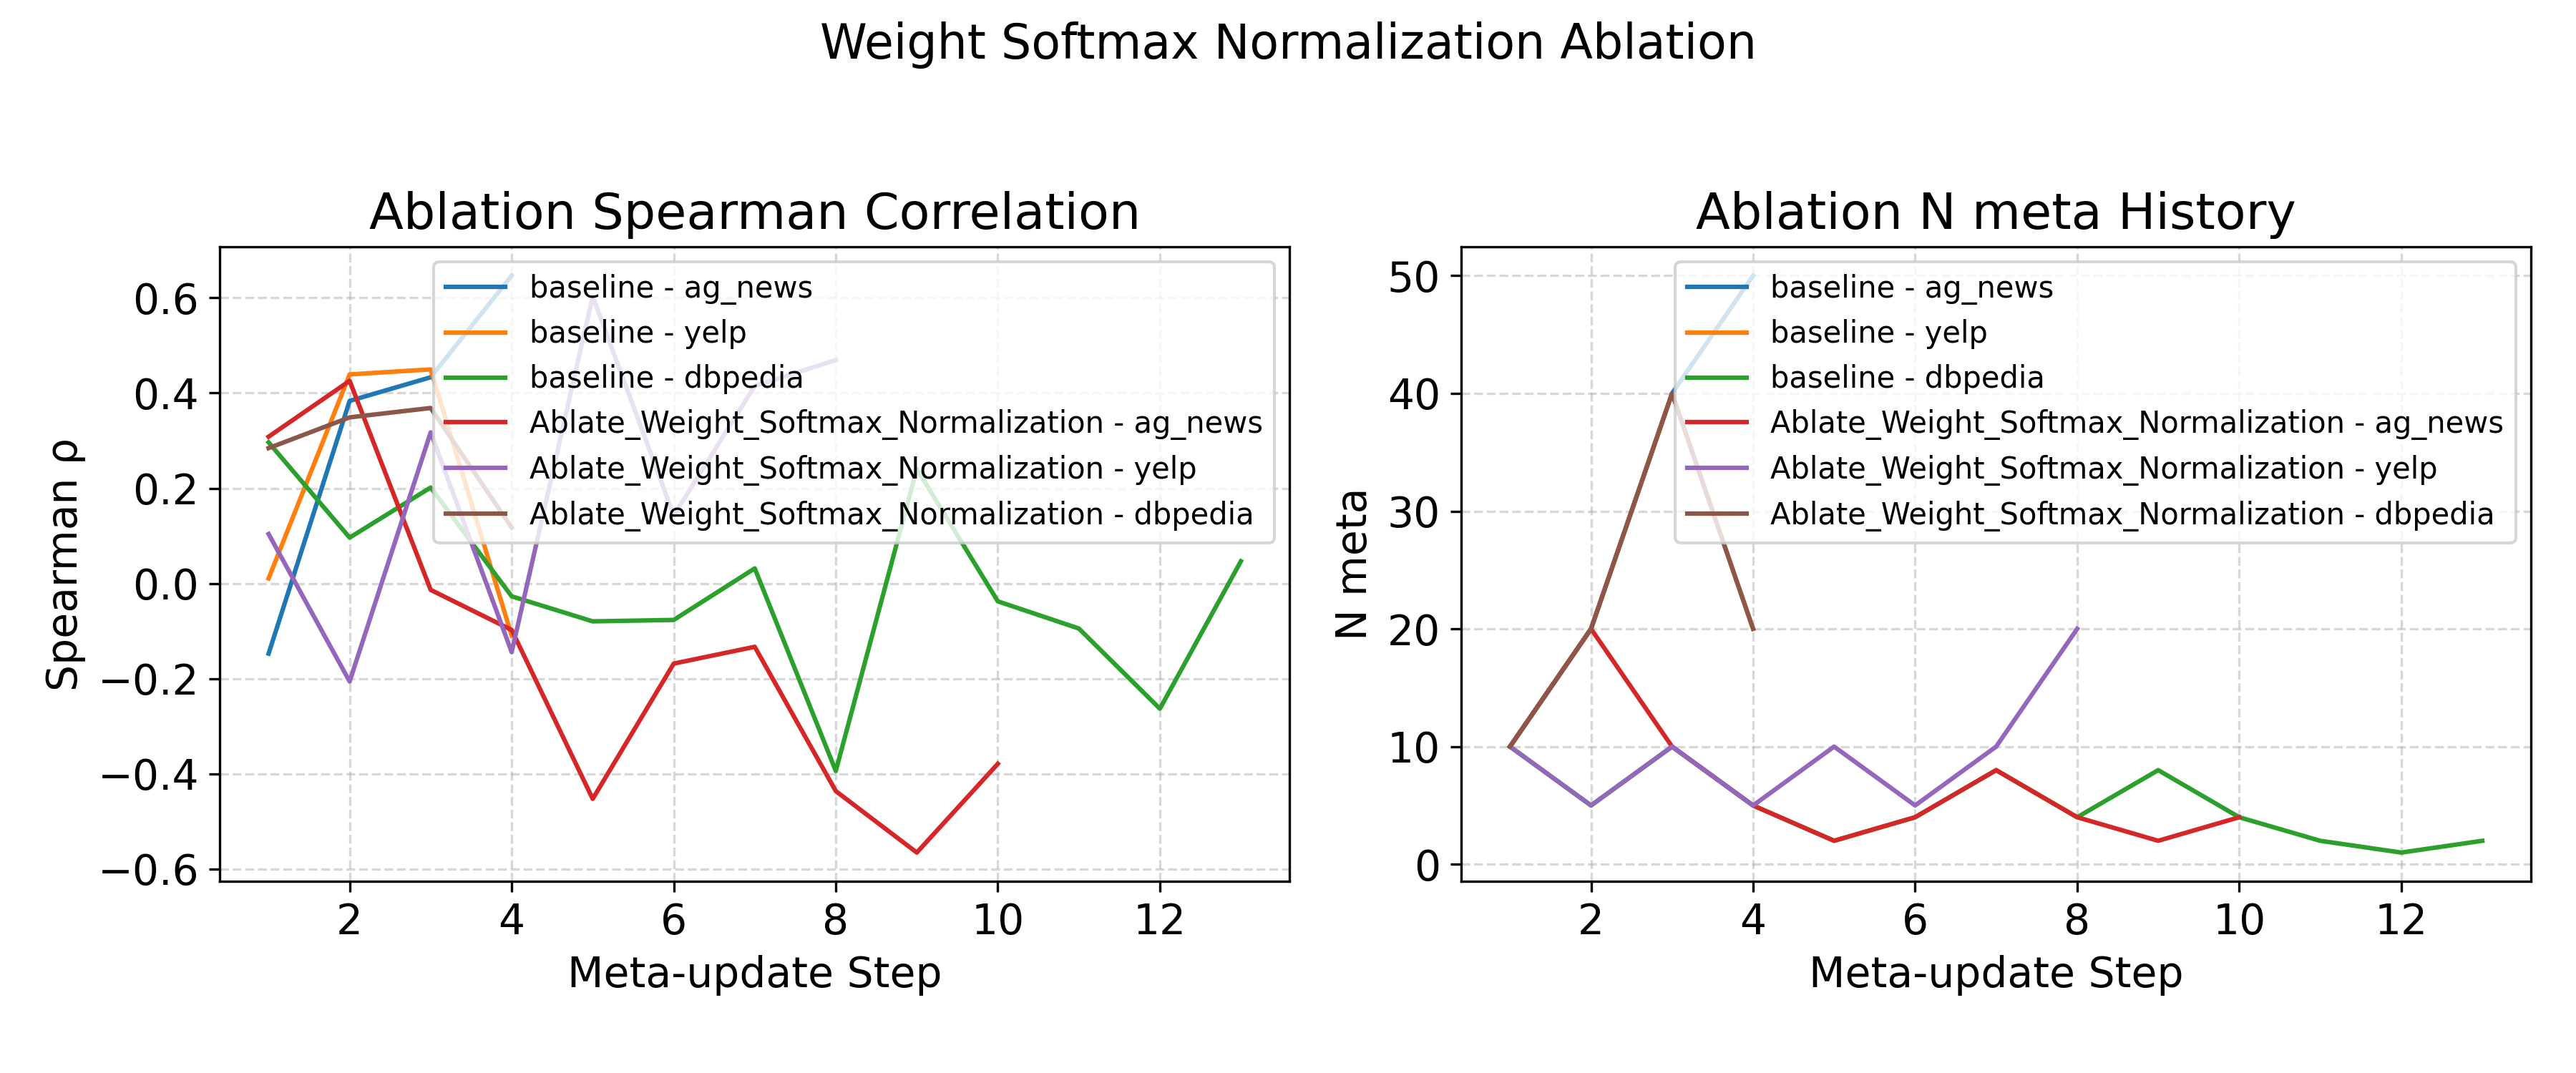
\includegraphics[width=0.48\linewidth]{ablate_weight_norm_summary.png}
  \caption{Ablation of softmax‐normalized weights: (a) Spearman collapse without softmax. (b) Spiking meta‐batch sizes. Softmax stabilizes training.}
  \label{fig:ablation-softmax}
\end{figure}

% --- Removed detailed multi‐panel figures from the main text to save space ---
% \begin{figure}[t]
%   ... classif_validation_metrics.png ...
% \end{figure}
% \begin{figure}[t]
%   ... classif_meta_dynamics.png ...
% \end{figure}
% \begin{figure}[t]
%   ... ablate_weight_norm_dynamics.png ...
% \end{figure}
% \begin{figure}[t]
%   ... ablate_weight_norm_meta_dynamics.png ...
% \end{figure}

\section{Discussion}
… highlight that some ablations (representation‐norm, label noise) were inconclusive (see App.~\ref{app:additional-ablations}) …

\section{Conclusion}
… main lessons and future directions …

% === Appendix (unlimited pages) ===
\appendix
\section{Additional Ablations}
\label{app:additional-ablations}

\begin{figure}[h]
  \centering
  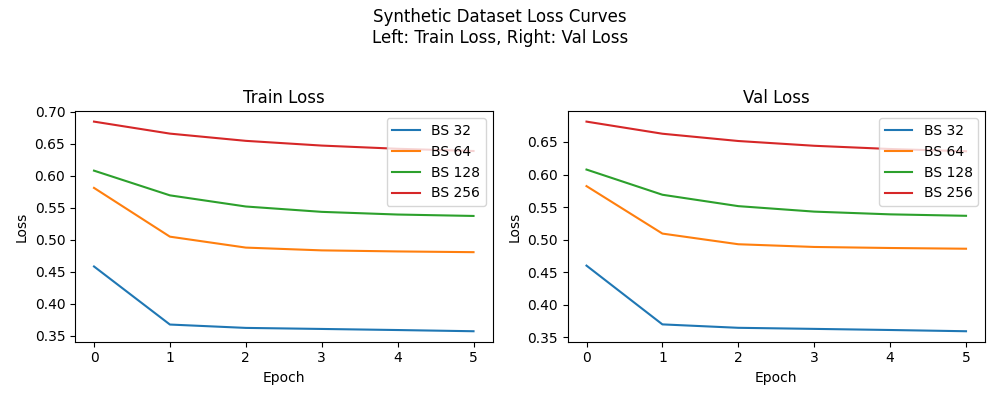
\includegraphics[width=0.48\linewidth]{synthetic_loss_curves.png}
  \includegraphics[width=0.48\linewidth]{synthetic_spearman_uncorr.png}
  \caption{(App.) Detailed multi‐budget loss curves and unsmoothed Spearman correlations.}
  \label{fig:synthetic-detailed}
\end{figure}

\begin{figure}[h]
  \centering
  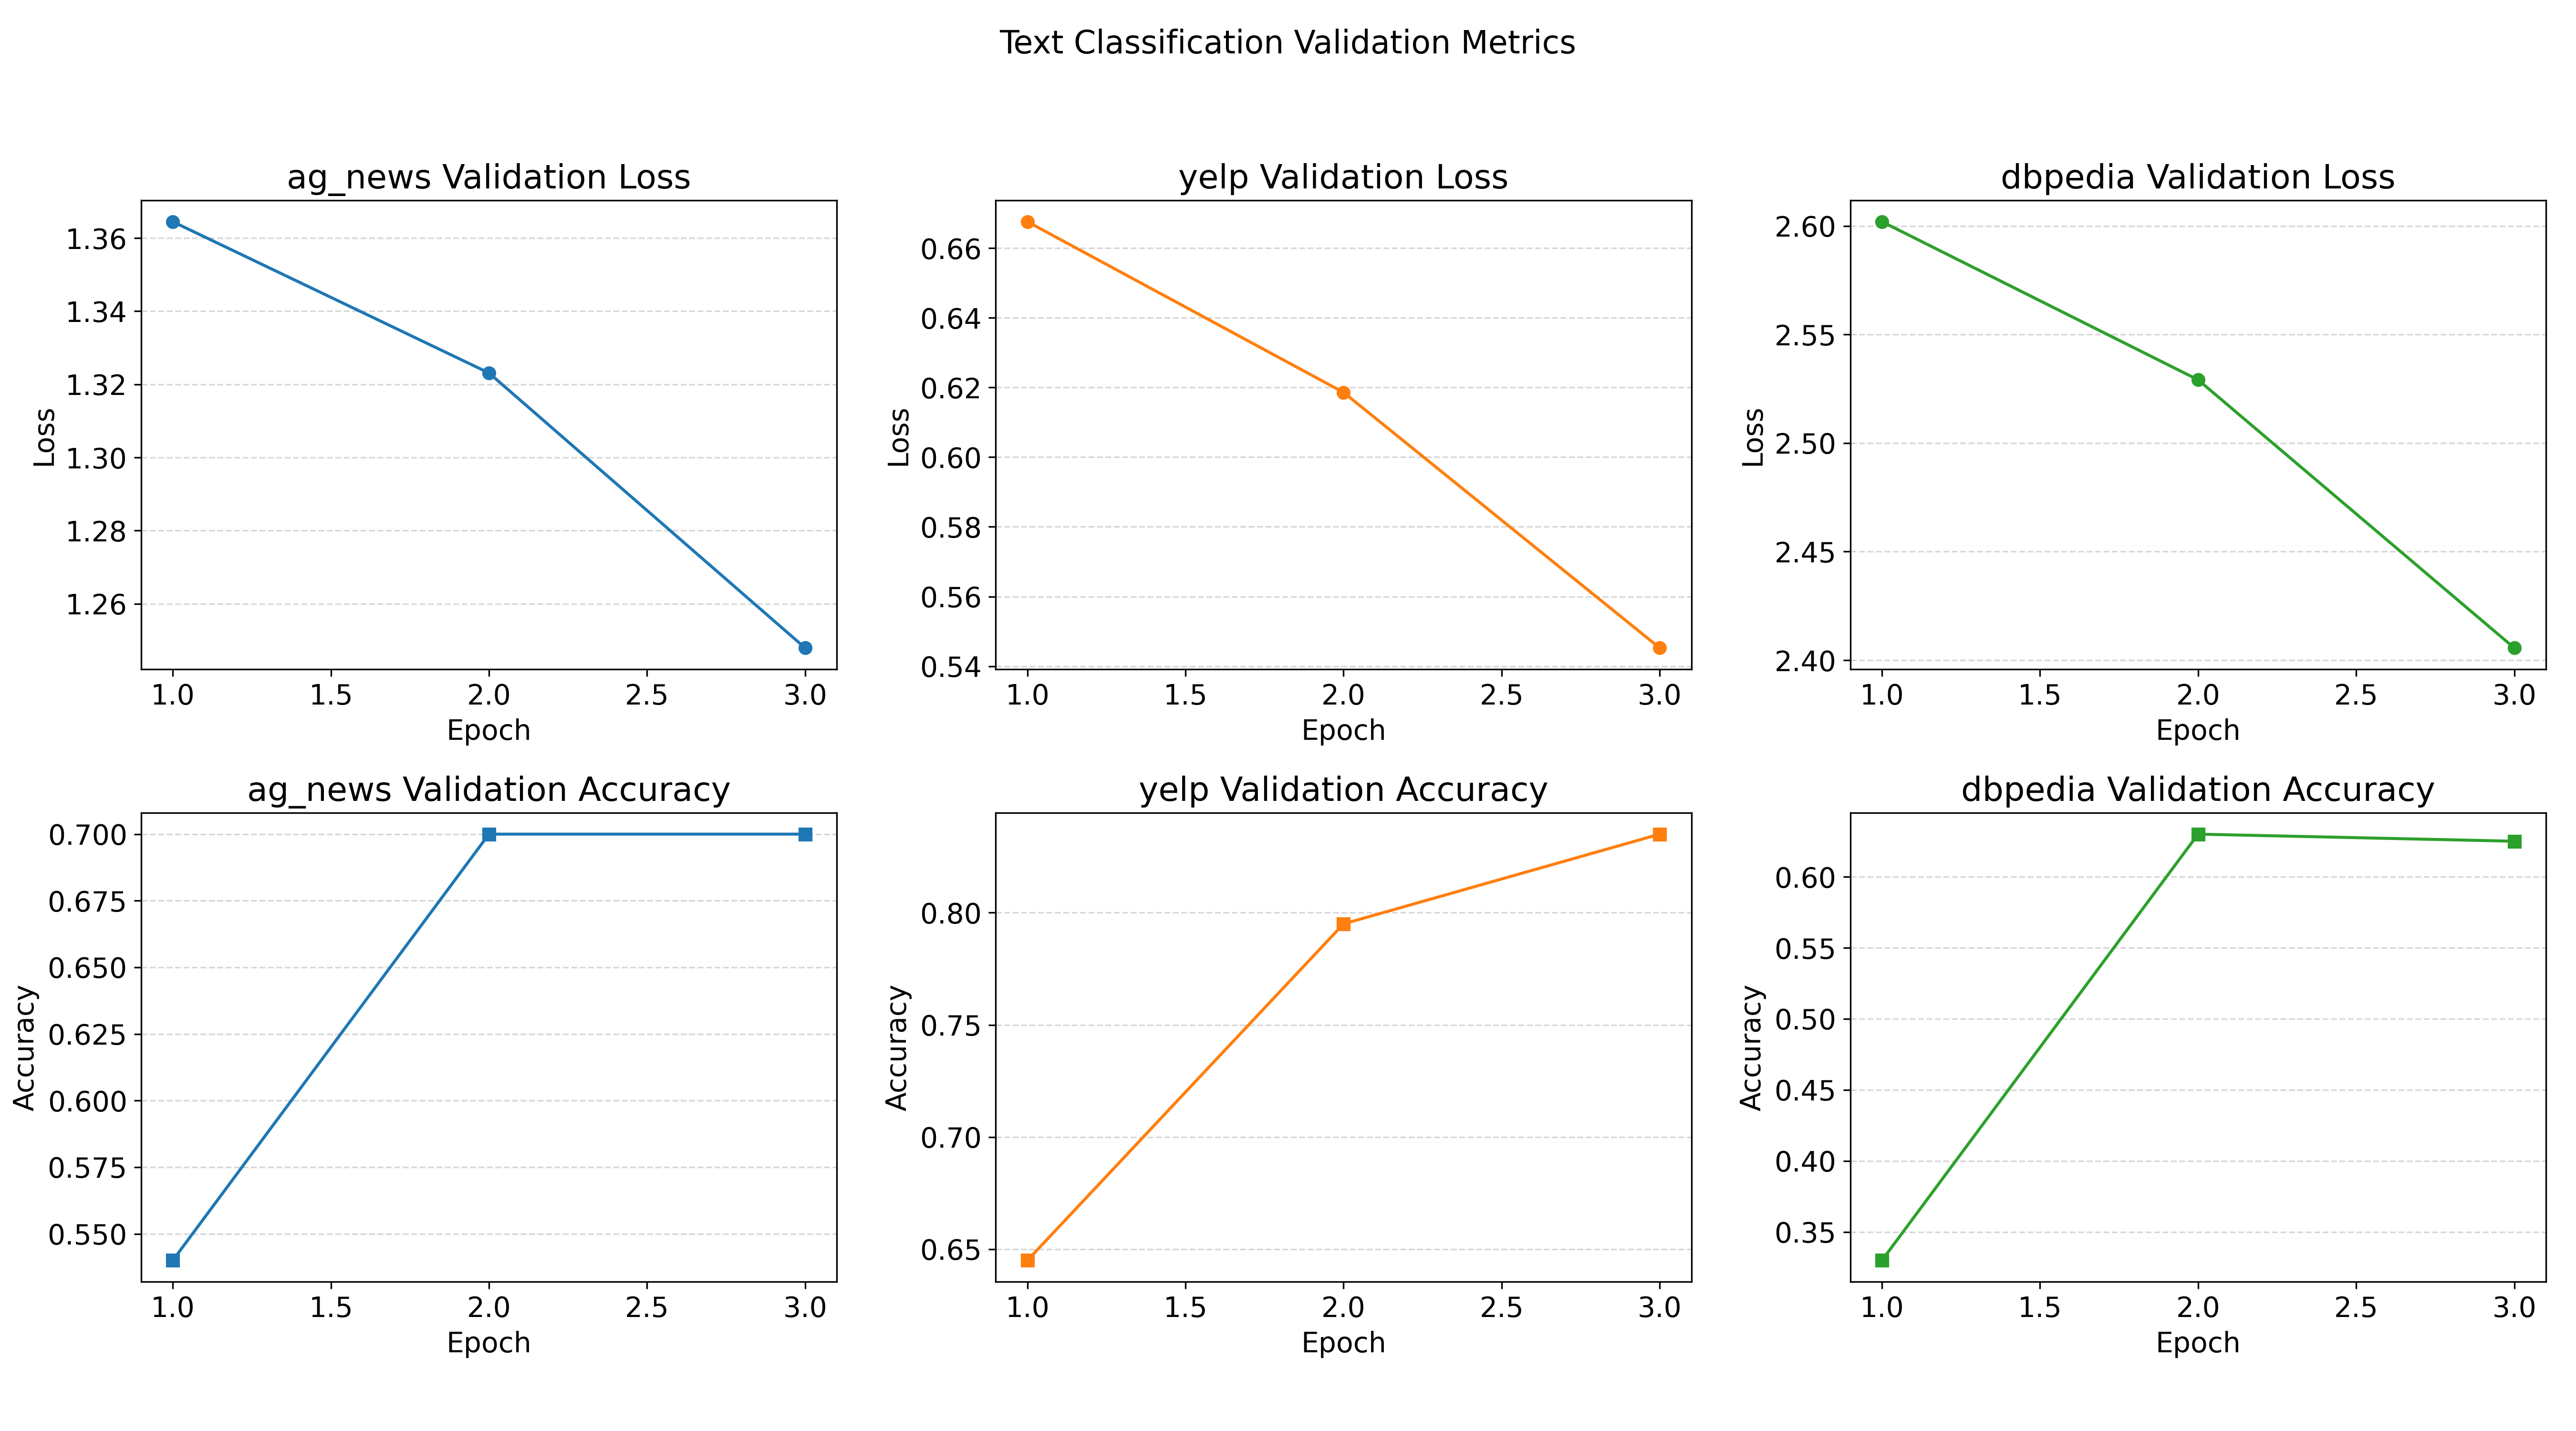
\includegraphics[width=0.48\linewidth]{classif_validation_metrics.png}
  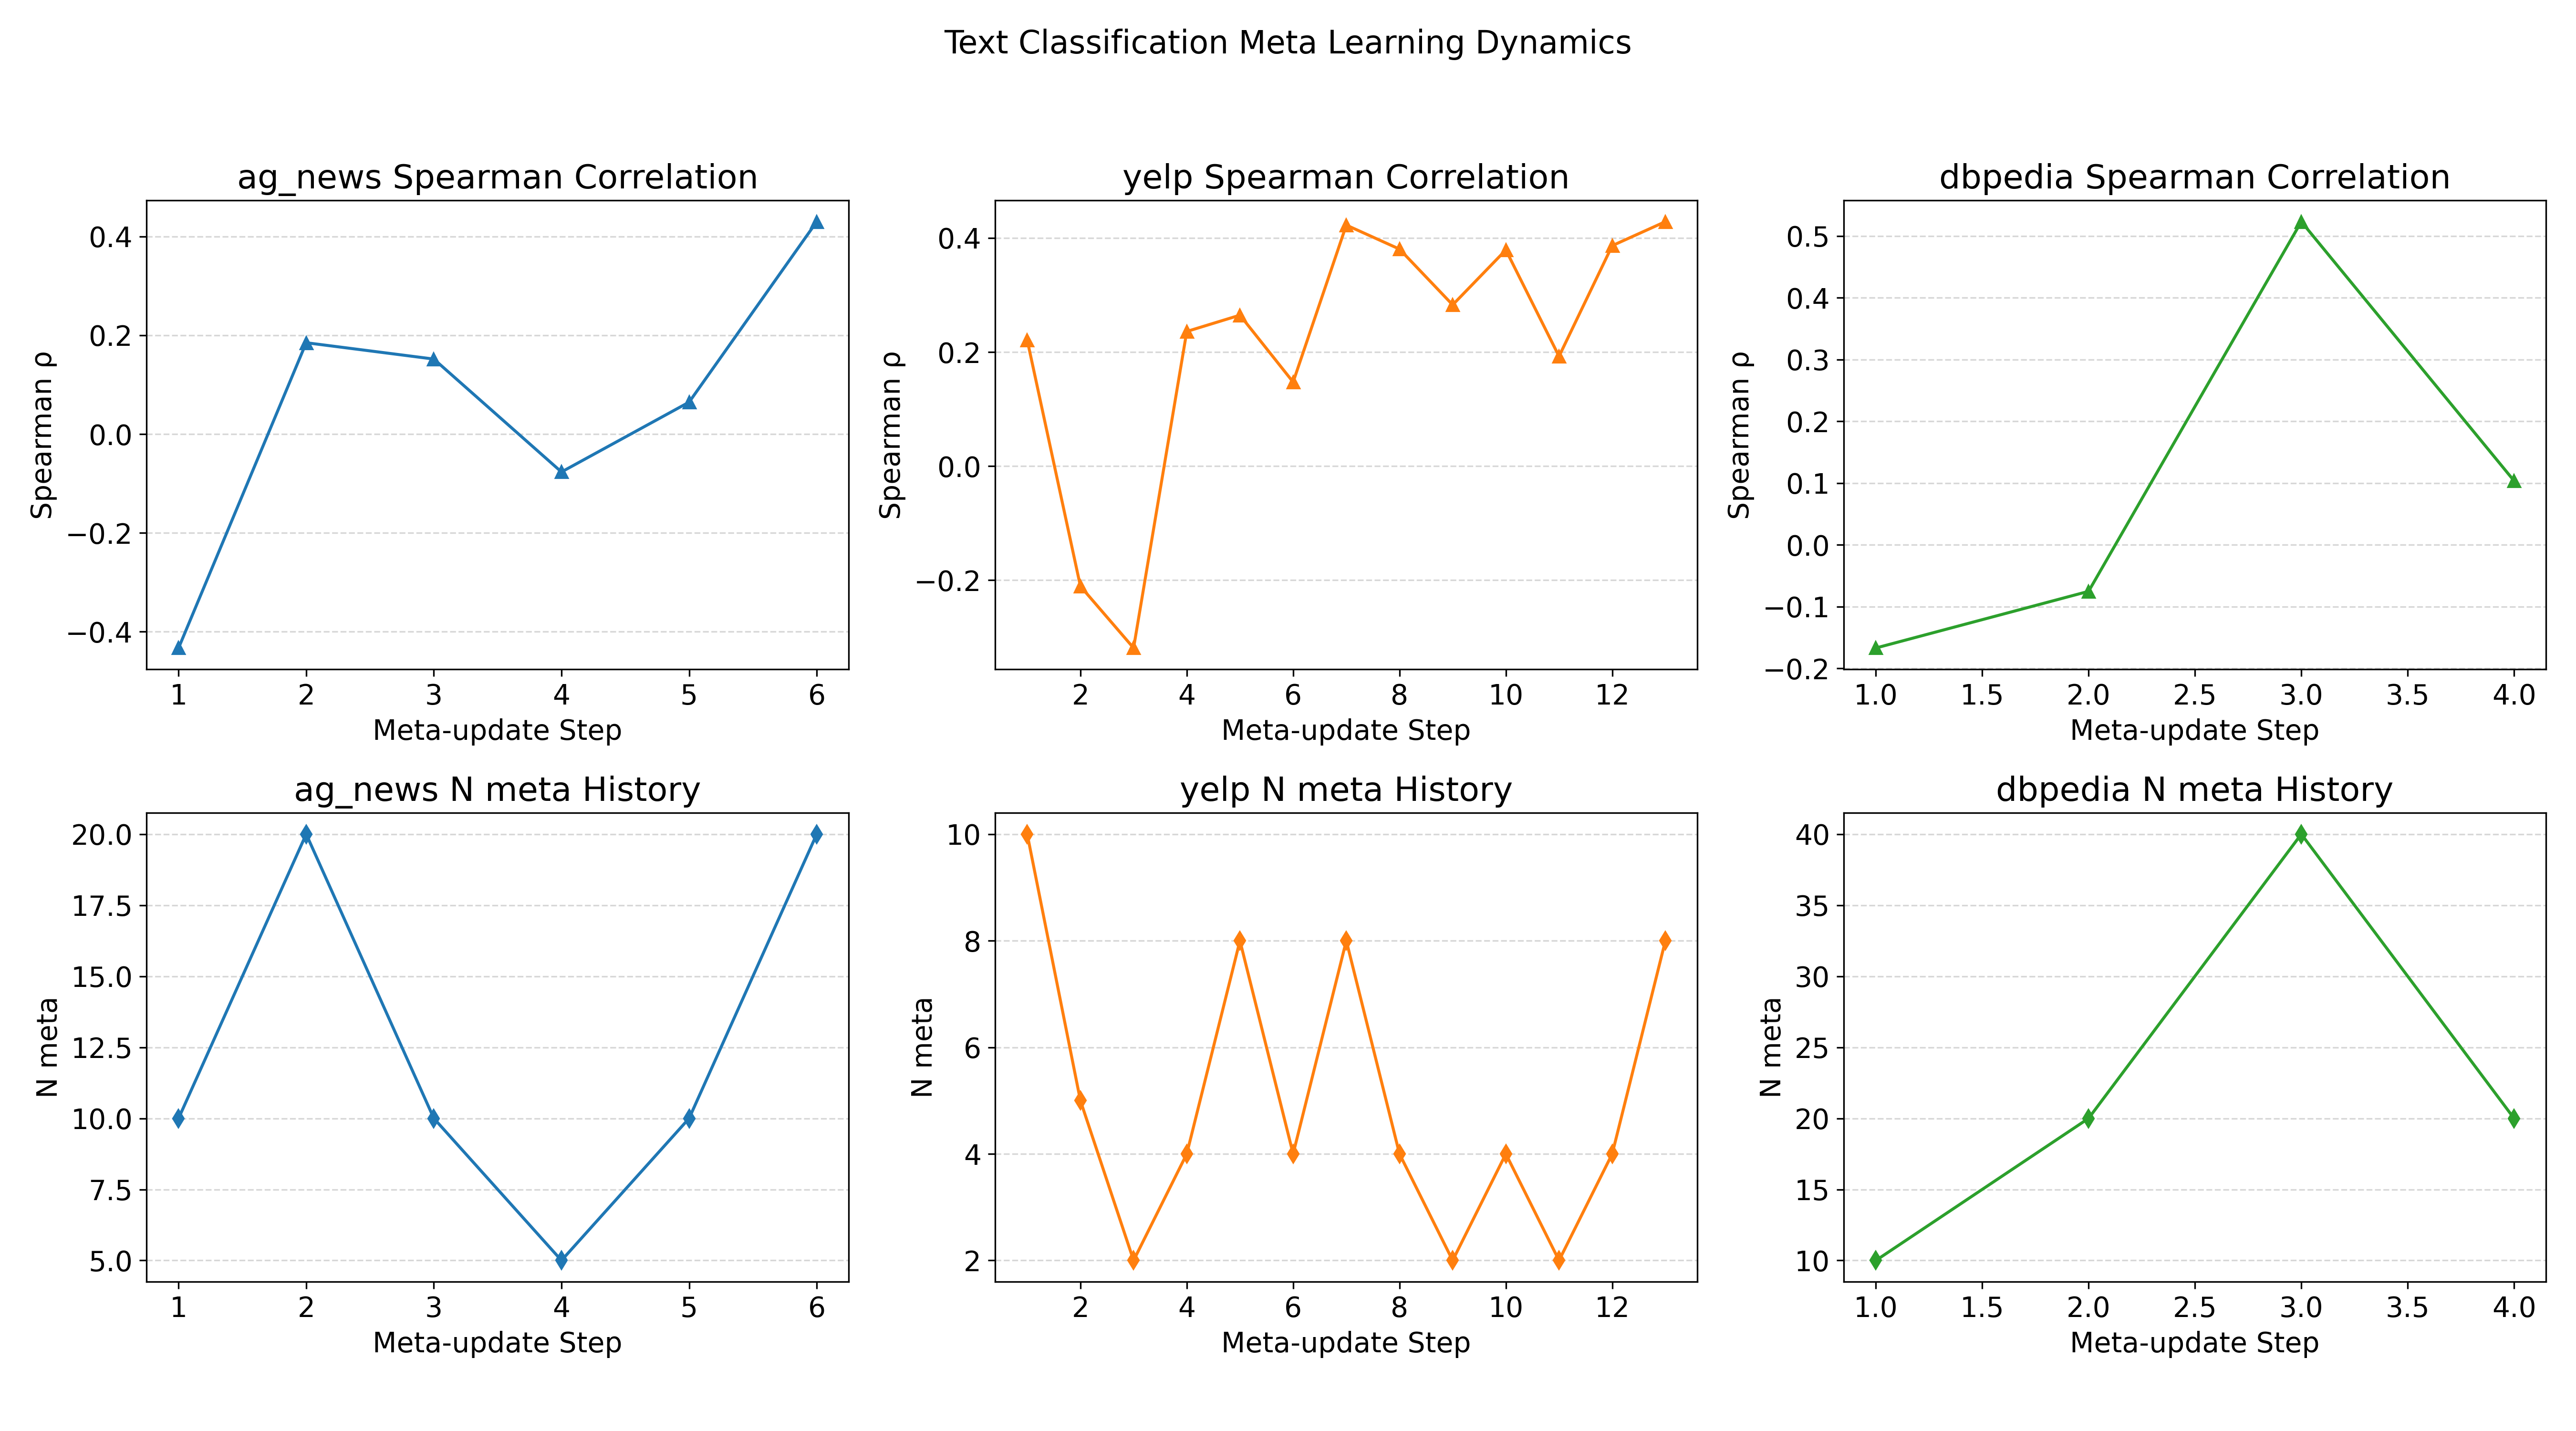
\includegraphics[width=0.48\linewidth]{classif_meta_dynamics.png}
  \caption{(App.) Per‐dataset validation curves and meta‐dynamics.}
  \label{fig:classif-detailed}
\end{figure}

\begin{figure}[h]
  \centering
  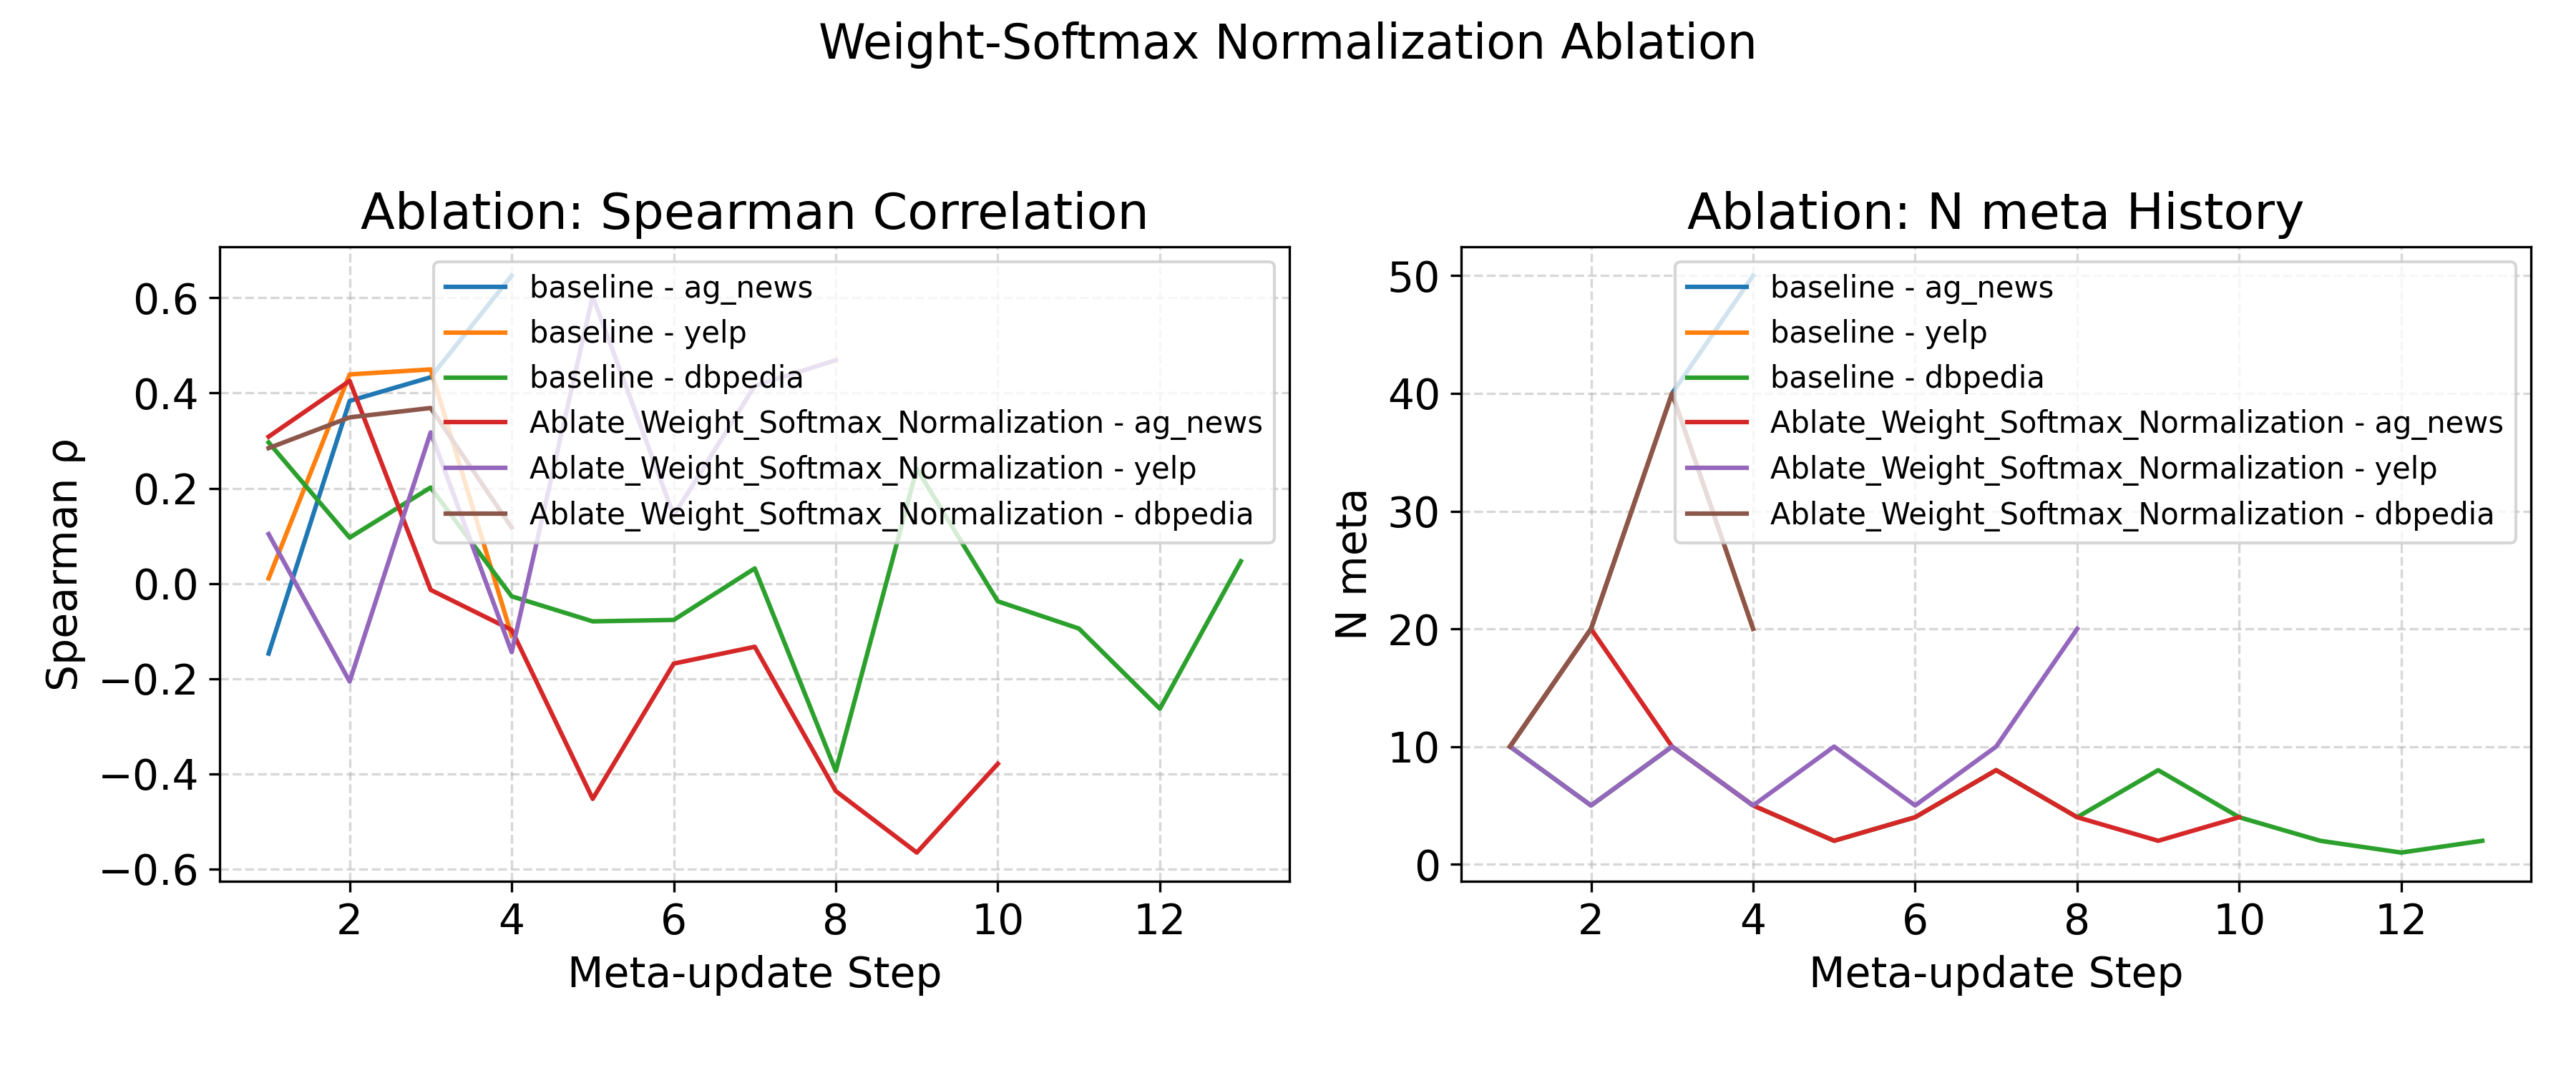
\includegraphics[width=0.48\linewidth]{ablate_weight_norm_dynamics.png}
  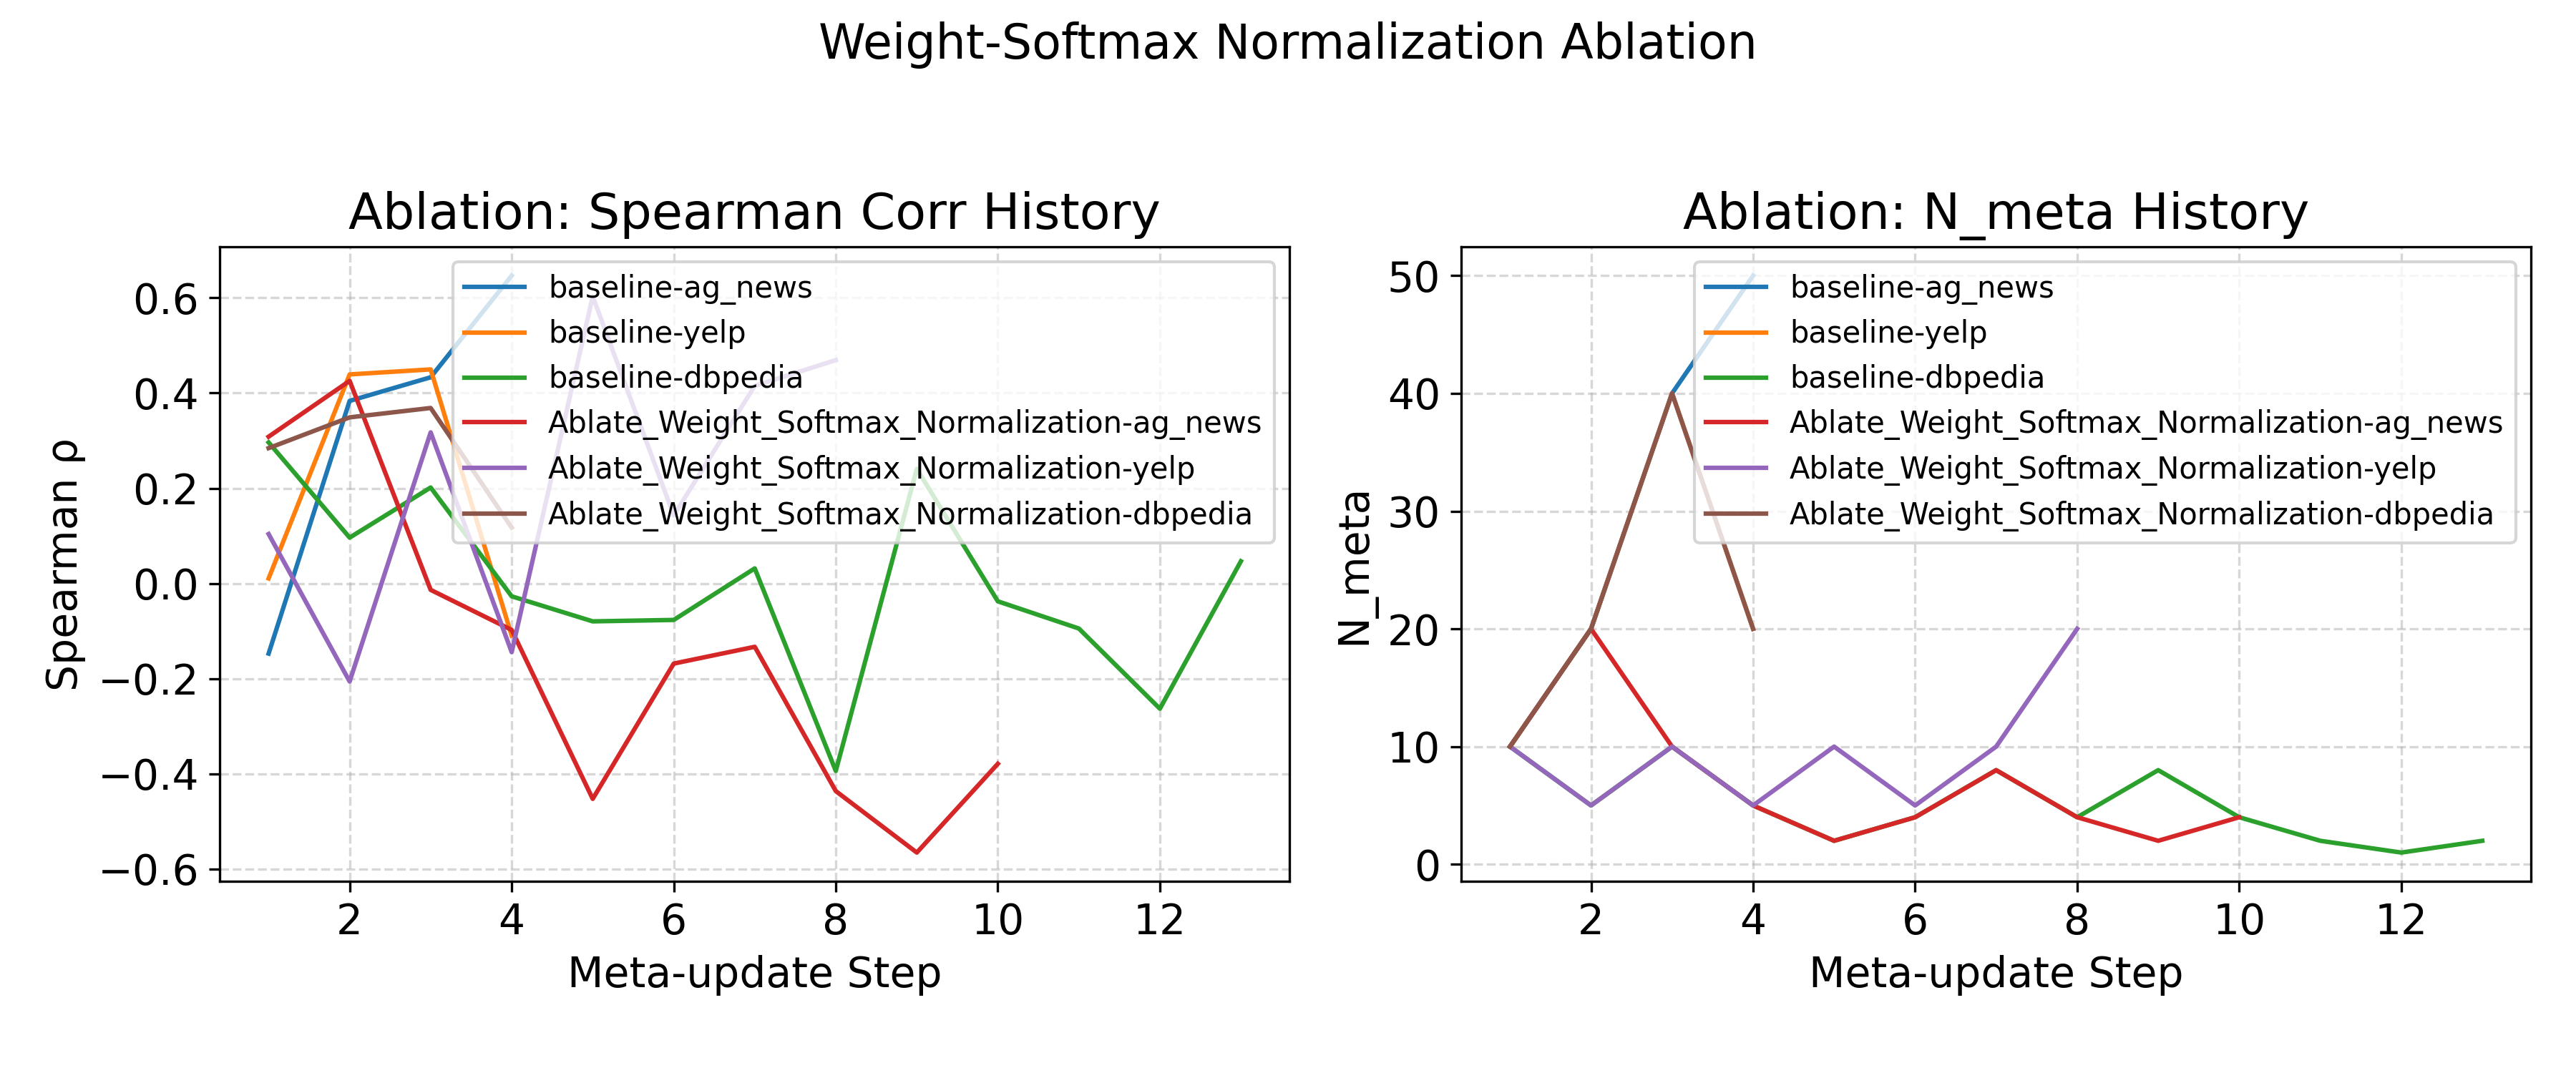
\includegraphics[width=0.48\linewidth]{ablate_weight_norm_meta_dynamics.png}
  \caption{(App.) Full dynamics of the weight‐softmax ablation.}
  \label{fig:ablation-softmax-detailed}
\end{figure}

\begin{figure}[h]
  \centering
  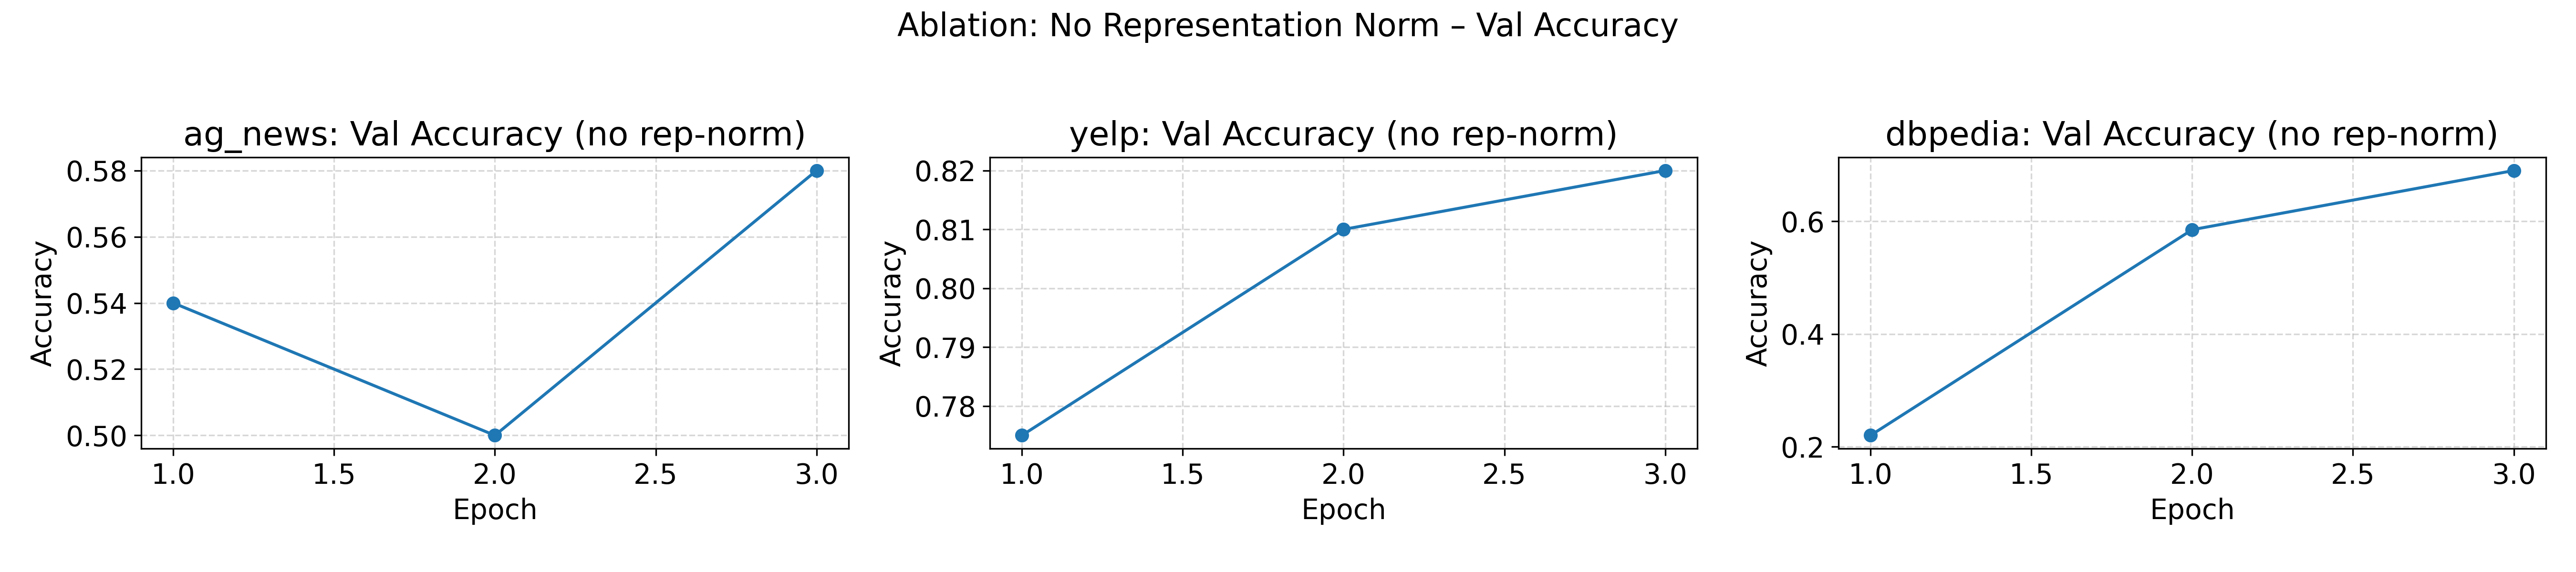
\includegraphics[width=0.48\linewidth]{ablate_no_repnorm_val_acc.png}
  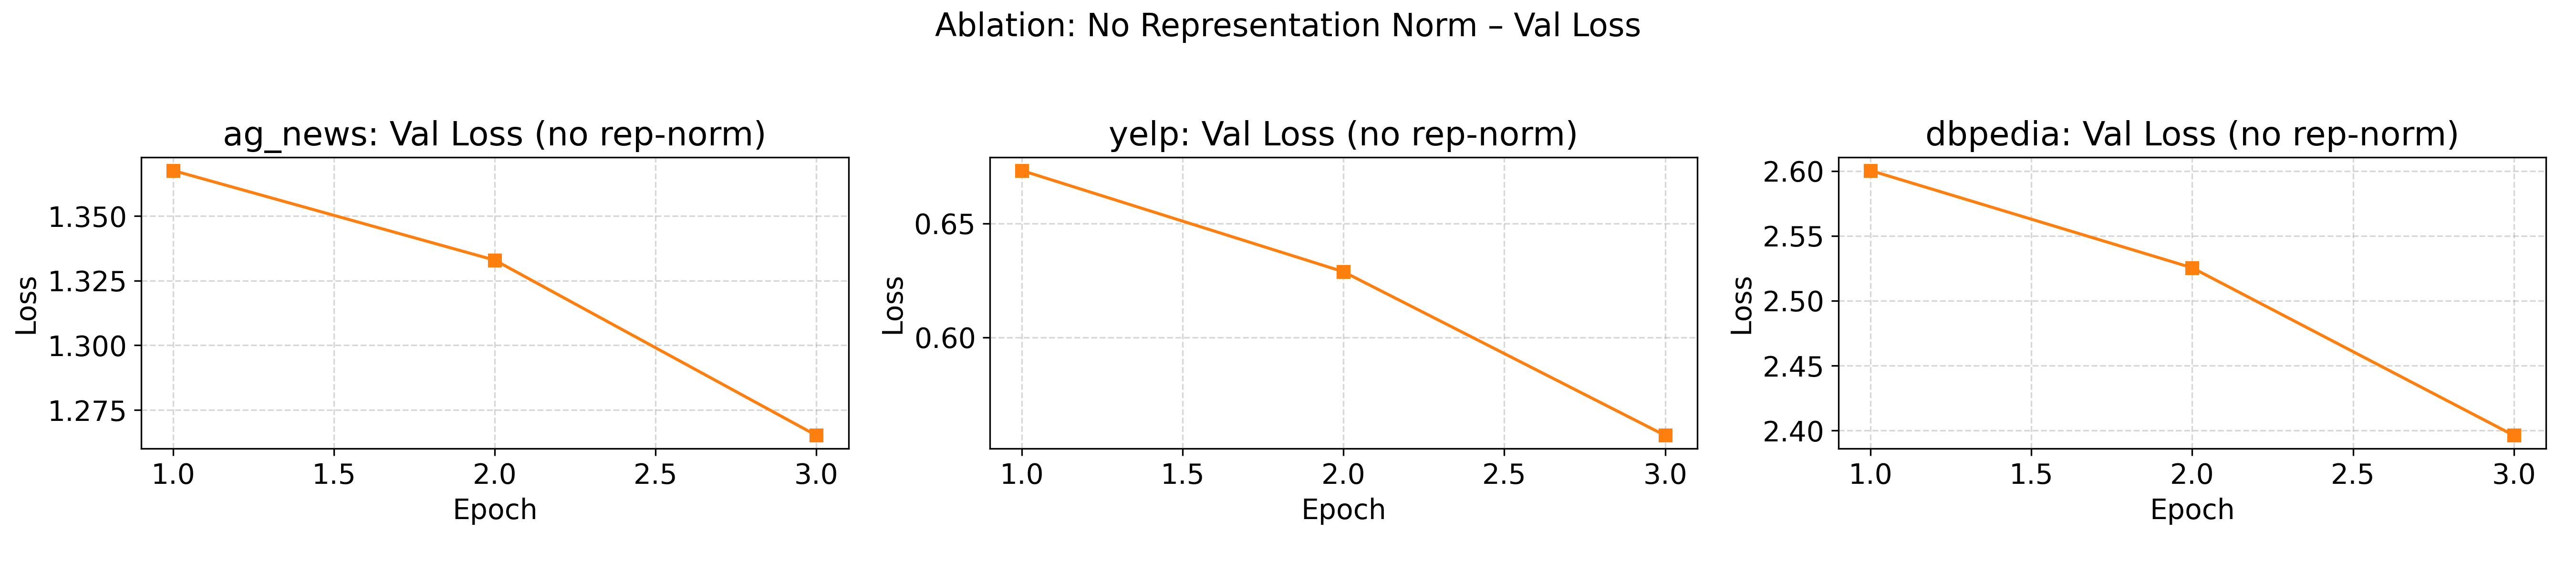
\includegraphics[width=0.48\linewidth]{ablate_no_repnorm_val_loss.png}
  \caption{(App.) Representation‐norm ablation on validation metrics.}
  \label{fig:ablation-repnorm}
\end{figure}

\begin{figure}[h]
  \centering
  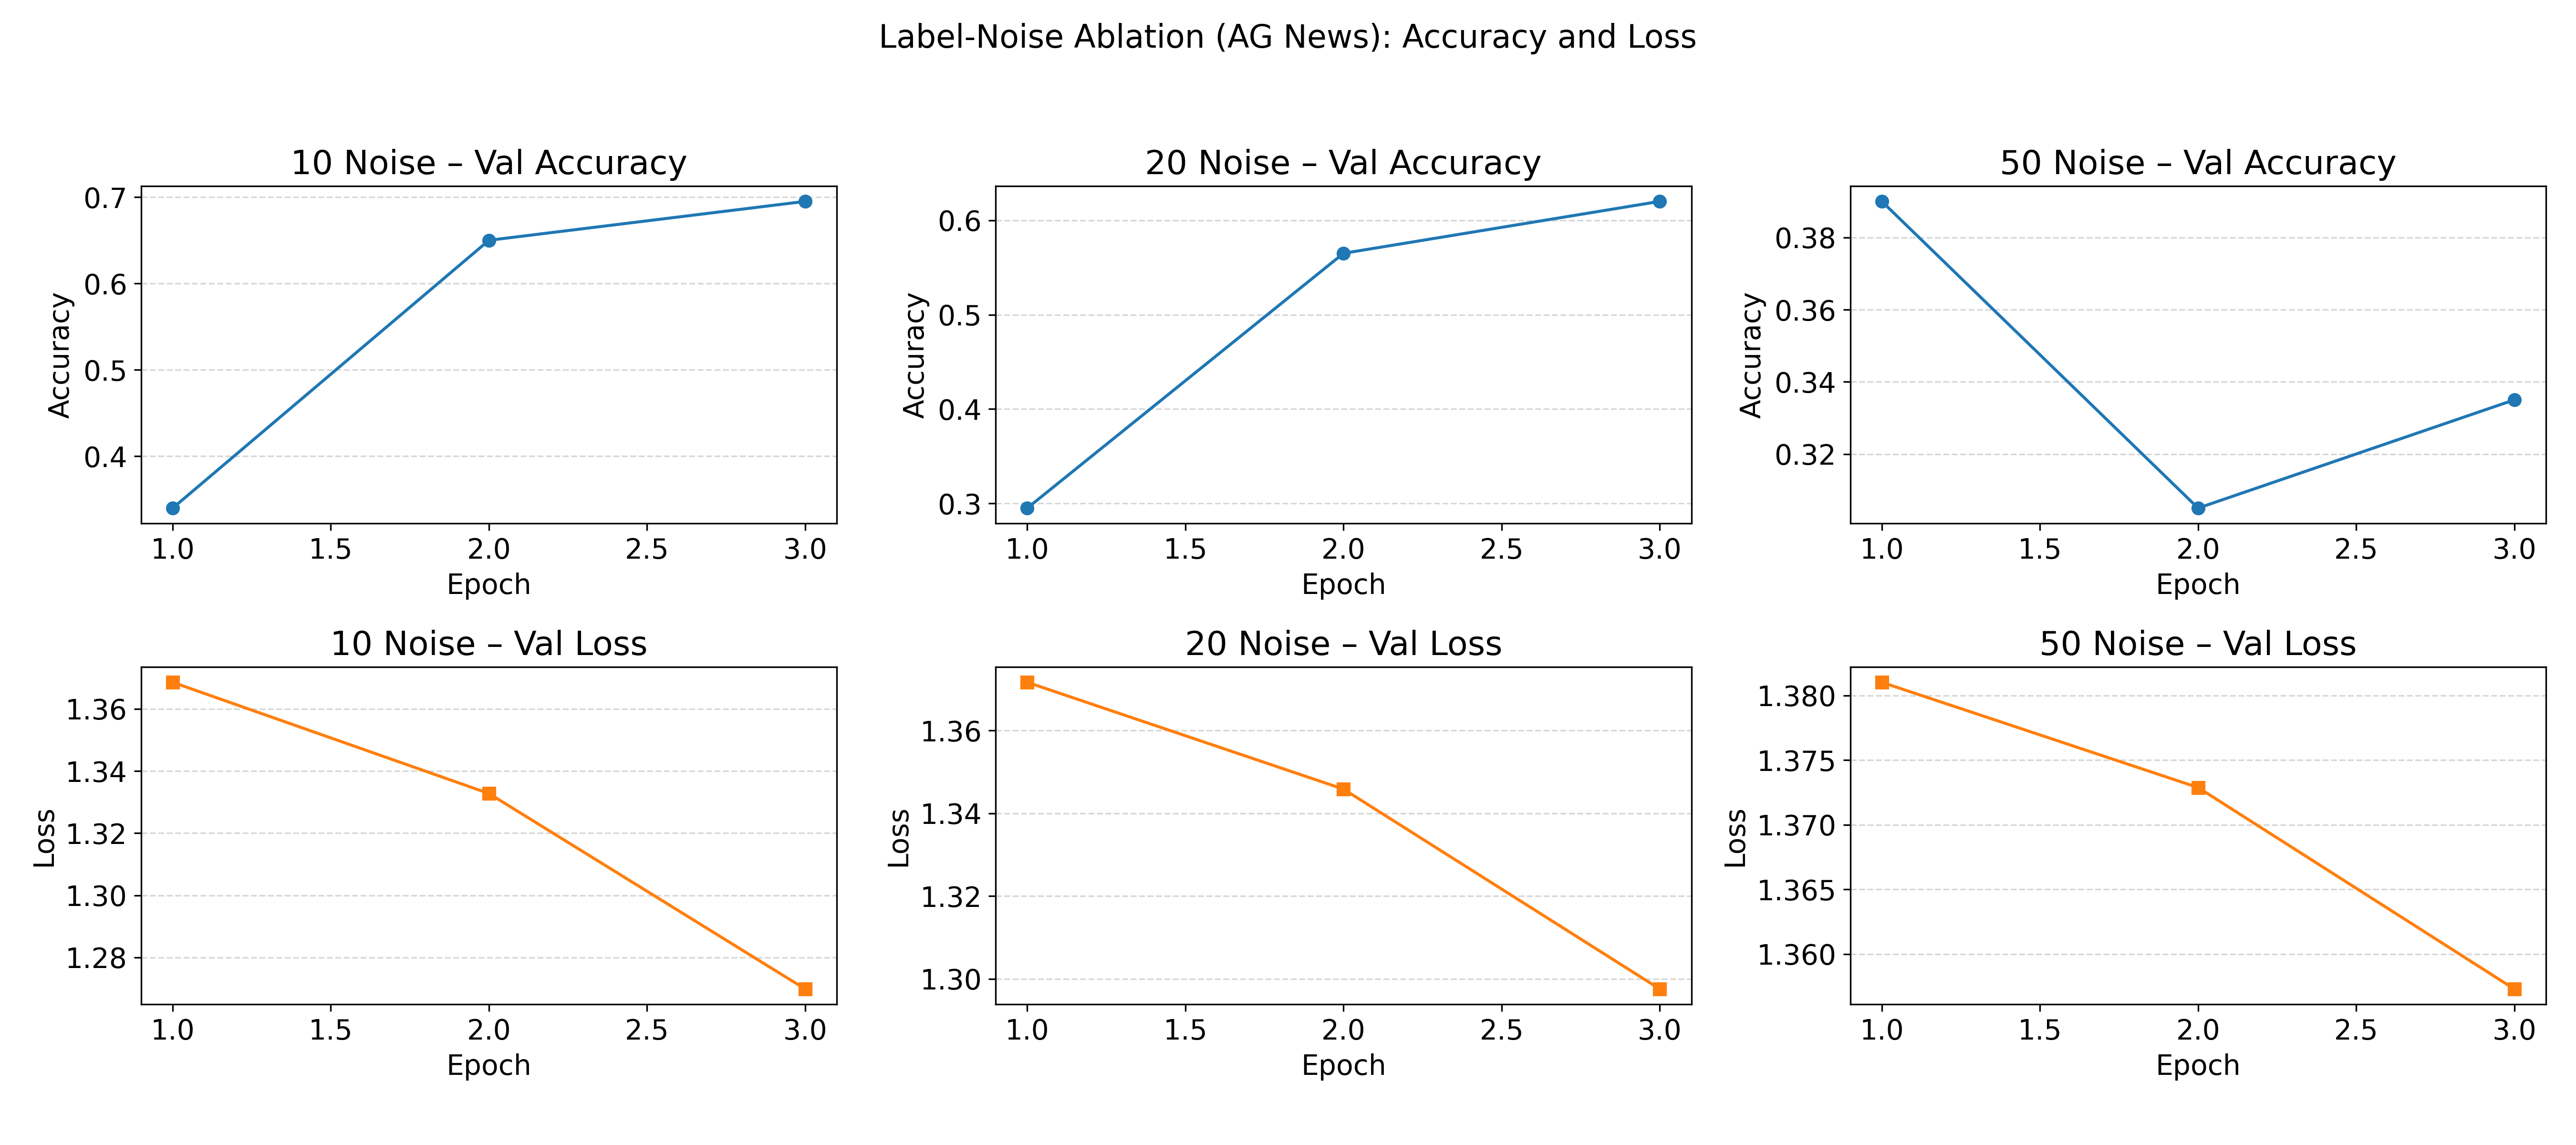
\includegraphics[width=0.48\linewidth]{ablate_label_noise_agnews_acc_loss.png}
  \includegraphics[width=0.48\linewidth]{ablate_label_noise_corr_meta.png}
  \caption{(App.) Label‐noise ablation: accuracy/loss and Spearman/meta‐batch plots.}
  \label{fig:ablation-labelnoise}
\end{figure}

\begin{filecontents}{references.bib}
@inproceedings{jiang2021data,
  title={Data valuation using optimized models},
  author={Jiang, Anthea and Kim, Melody Y and Gupta, Ming and Oh, Jamie},
  booktitle={ICML},
  year={2021}
}
@inproceedings{sener2018active,
  title={Active learning for convolutional neural networks: A core‐set approach},
  author={Sener, Ozan and Savarese, Silvio},
  booktitle={ICLR},
  year={2018}
}
@inproceedings{alain2016variance,
  title={Variance reduction in SGD by distributed importance sampling},
  author={Alain, Guillaume and Lamb, Alexandre and et al.},
  booktitle={arXiv},
  year={2016}
}
@inproceedings{kendall2018multi,
  title={Multi‐task learning using uncertainty to weigh losses for scene geometry and semantics},
  author={Kendall, Alex and Gal, Yarin and Cipolla, Roberto},
  booktitle={CVPR},
  year={2018}
}
@inproceedings{gao2019consistency,
  title={Consistency‐based semi‐supervised active learning: Initial explorations},
  author={Gao, Yijun and Snoek, Cees GM and Welling, Max},
  booktitle={arXiv},
  year={2019}
}
\end{filecontents}

\end{document}